\documentclass[11pt,a4paper]{article}
\usepackage{graphicx}
\usepackage{amsfonts}
\usepackage[utf8]{inputenc}
\usepackage[a4paper, total={6.5in, 9in}]{geometry}
\usepackage{amsthm}
\usepackage{amssymb}
\usepackage{hyperref}
\usepackage{caption}
\usepackage{indentfirst}
\usepackage[]{algorithm2e}
\usepackage{amsmath}
\usepackage{algorithm,algorithmic}
\usepackage{algpseudocode}
\usepackage[superscript,biblabel]{cite}

\hypersetup{
    colorlinks,
    linkcolor  = black,
    citecolor = black
 }
 
\makeatletter
\renewcommand\paragraph{\@startsection{paragraph}{4}{\z@}%
            {-2.5ex\@plus -1ex \@minus -.25ex}%
            {1.25ex \@plus .25ex}%
            {\normalfont\normalsize\bfseries}}
\makeatother
\setcounter{secnumdepth}{4}
\setcounter{tocdepth}{4}

\renewcommand{\figurename}{Figura}
\addto\captionsenglish{\renewcommand{\figurename}{Figura}}

\makeatletter
\renewcommand{\ALG@name}{Algoritmo}
\makeatother

\theoremstyle{plain}
\setlength{\footskip}{90pt}

\newenvironment{algoritmo}[1][htb]
  {\renewcommand{\algorithmcfname}{Algoritmo}% Update algorithm name
   \begin{algorithm}[#1]%
  }{\end{algorithm}}

\begin{document}

\begin{titlepage}
	\centering

	\begin{figure}[htp]
	\centering
	\includegraphics[scale=.3]{logo-unc.jpeg}
	\end{figure}
	
	{\scshape\Large\textsc{Universidad Nacional de Córdoba} \par}
	\vspace{0.5cm}
	{\scshape\large FaMAF\par}
	\vspace{1.5cm}

	{\LARGE\bfseries Matemática Discreta II\par}
	\vspace{.7cm}
	{\Large Proyecto: Primera Parte\par}
	\vspace{3cm}
	{\Large\scshape{Esteban L. Boucher}\par}
	\vspace{.4cm}
	{\large\ttfamily eboucher7@gmail.com\par}
	\vspace{.4cm}
	{\large Septiembre 2016}
	\vfill
	Prof.~Daniel \textsc{Penazzi}

	\date{Septiembre, 2016}
\end{titlepage}

\renewcommand\refname{}

\renewcommand{\contentsname}{Índice general}

\tableofcontents
\newpage
\section{Introducción}

	\subsection{Motivación del proyecto}

 El problema de coloreo de grafos consiste en asignar colores a ciertos elementos de un grafo sujetos a ciertas restricciones.

 El problema de coloreo de vértices es el problema más común de coloreo de grafos. El problema es, dados m colores, encontrar una forma de colorear los vértices de un grafo de tal manera que no hayan dos vértices adyacentes utilizando el mismo color.
 
 El interés acerca de este problema se debe a su gran número de aplicaciones. Entre las más conocidas de coloreo de grafos se destacan\cite {1}:
 
\begin{itemize}

\item{\textbf{{{{Establecer horarios y cronogramas}}}}}

Supongamos que queremos hacer un cronograma de exámenes para un universidad. Listamos diferentes asignaturas y estudiantes matriculados en cada asignatura. Muchas asignaturas tendrán estudiantes en común. \emph{¿Cómo se puede organizar el cronograma de modo que no hayan dos exámenes con un estudiante en común programados al mismo tiempo? ¿Cuántas ranuras de tiempo mínimo son necesarias para programar todos los exámenes?} Este problema se puede representar como un grafo en el que cada vértice es una asignatura y una arista entre dos vértices significa que hay un estudiante común. Este es un problema de coloreo de grafos, donde el número mínimo de intervalos de tiempo es igual al número cromático del grafo.

\item{\textbf{{{Asignación de frecuencias de radio móvil}}}}

Cuando se asignan frecuencias a las torres, las frecuencias asignadas a todas las torres que se encuentran en el mismo lugar debe ser diferentes. ¿Cómo asignar frecuencias con esta restricción? ¿Cuál es el mínimo numero de frecuencias necesarias? Este problema es también un ejemplo del problema de coloreo de grafos donde cada torre representa un vértice y una arista entre dos torres representa que están en el rango de la otra.

\item{\textbf{{{Sudoku}}}}

El suduku es también una variación del problema de coloreo de grafos en el cual cada celda representa un vértice. Hay una arista entre dos vértices si están en la misma fila o la misma columna o el mismo bloque.

\item{\textbf{{{Asignación de registros}}}}

En optimización de compiladores, la asignación de registros es el proceso de asignar un gran número de variables del programa de destino a un número reducido de registros de la CPU. Este problema también un problema de coloreo de grafos.

\item{\textbf{{{Grafos bipartitos}}}}

Podemos comprobar si un grafo es bipartito o no coloreando el grafo utilizando dos colores. Si un grafo dado es 2-coloreable, entonces es bipartito, de lo contrario no lo es. 
 
\item{\textbf{{{Mapa de coloreo}}}}

Mapas gráficos de países o provincias donde dos ciudades adyacentes no pueden ser asignadas con el mismo color. Cuatro colores son suficientes para colorear cualquier mapa\cite {2}.

\end{itemize}
 
 El siguiente programa consiste en la resolución de ese problema.

	\subsection{Propósito y objetivos}

Actualmente no se conoce un algoritmo de tiempo polinomial que resuelva el problema de coloreo de grafos. Sin embargo, hay una cierta calidad mínima que se puede obtener. Supongamos que \emph{d} es el mayor grado de cualquier vértice en nuestro grafo. A medida que avanzamos en el coloreo, cuando coloreamos cualquier vértice particular \emph{v}, este está unido a lo sumo con otros \emph{d} vértices, de los cuales algunos pueden ya estar coloreados. Luego, hay a lo sumo \emph{d} colores que hay que evitar usar. Usamos el color de menor número no prohibido. Esto significa que usamos colores numerados \emph{d}+1 o menor, dado que al menos uno de los colores 1, 2, ..., \emph{d}+1 NO está prohibido. De esta manera, nunca necesitamos usar ningún color de mayor número que \emph{d}+1. Esto nos da el siguiente teorema:

\subsubsection{Coloreo Greedy}
\newtheorem*{Teorema*}{Teorema 1 (Coloreo Greedy)}

\begin{Teorema*}
Si d es el mayor de los grados de los vértices en un grafo G, entonces G tiene una coloración propia con d + 1 colores o menos, es decir, el número cromático de G es como máximo d + 1.
\end{Teorema*}

 Esto nos da una cota superior del número cromático del grafo\cite {4}.\\

El objetivo de este proyecto consiste en cargar un grafo y dar un coloreo propio de sus vértices, corriendo repetidamente Greedy usando ordenes que cumplan con el Teorema 1.

	\subsection{Restricciones}

\begin{itemize}

\item\textbf{{Tiempo}}

El presente programa está estipulado para ser razonablemente rápido. En particular, con todos los grafos de ejemplo probados por la cátedra\cite{5}\cite{6}, se espera que termine en menos de una hora. Algunos de esos grafos pueden llegar a tener cerca de 2 millones de vértices y 10 millones de aristas.

\item\textbf{{Memoria}}

El programa nunca debe usar más de 256 MB de memoria RAM.

\end{itemize}

\section{Formato del archivo de entrada}
\label{sec:2}

El formato de entrada es una variación de DIMACS, un formato estándar para representar grafos.
La descripción oficial de DIMACS es como sigue:

1. Ninguna línea tiene más de 80 caracteres.

2. Al principio hay cero o más líneas que empiezan con 'c' (sin las comillas), las cuales son líneas de comentario y son ignoradas.

3. Luego hay una línea de la forma:

p edge n m

donde n y m son dos enteros. n representa el número de vértices y m el número de lados.

4. Luego siguen m líneas todas comenzando con 'e' (sin las comillas) y dos enteros, representando un lado. Luego de esas m lineas se detiene la carga.

\newpage


\section{Estructura del programa}

En la Figura 1 se muestra un diagrama de la estructuración del programa en los distintos archivos.\\ 

\begin{figure}[htp]
\centering
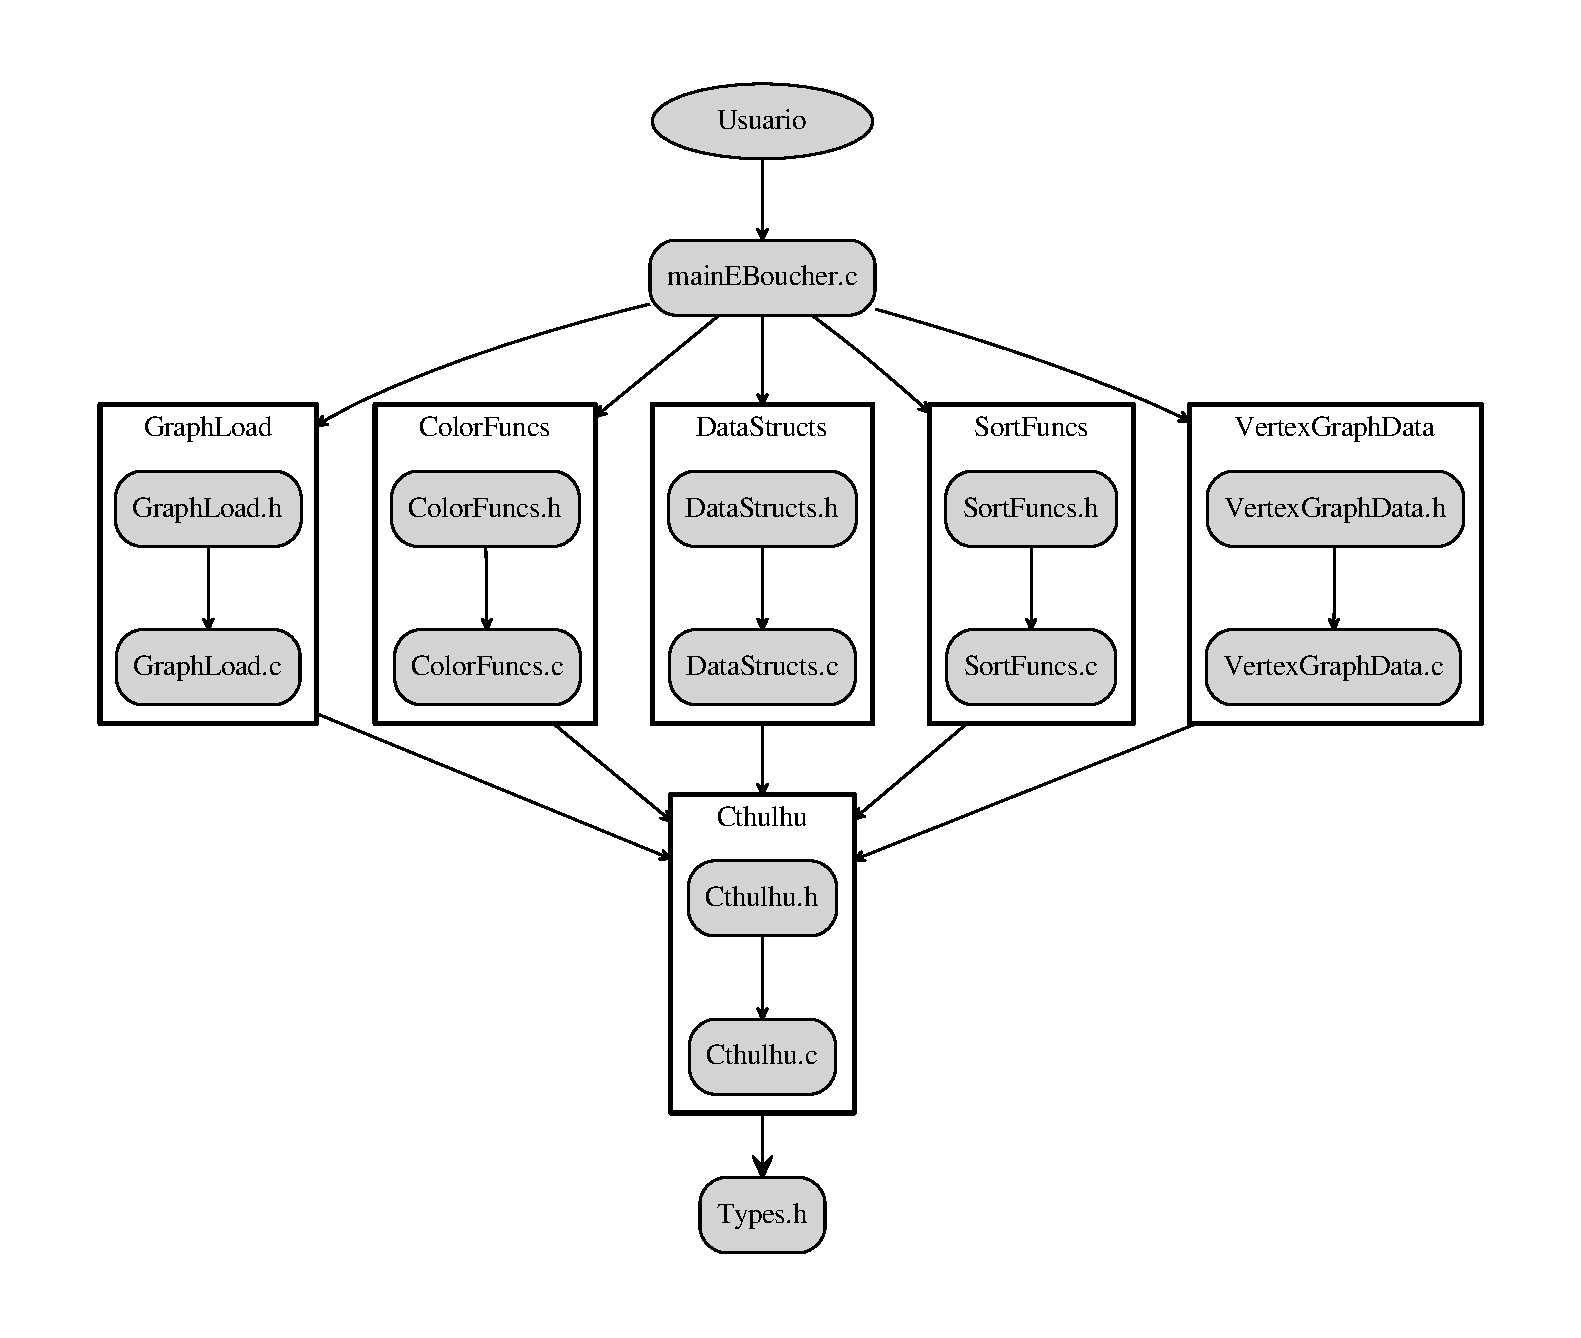
\includegraphics[scale=0.65]{diagram.pdf}
{\caption{Diagrama de archivos del programa}}
\label{fig:1}
\end{figure}

	\subsection{Descripción de estructuras y variables}
	\label{sec:3.1}
	
		\subsubsection{\texttt{struct \_NimheSt\_t}}
	
Las estructura principal de este programa es \texttt{struct \_NimheSt\_t}, la cual contiene toda la información del grafo necesaria para correr el algoritmo de Greedy y obtener del mismo para modificar el orden de los vértices acorde a las distintas funciones de ordenación.\\

\newpage
\begin{itemize}
\item\textbf{{Información básica del grafo}}\\

 \texttt{NimheSt} contiene la cantidad de vértices y lados del grafo cargado y la cantidad de colores que está usando en el momento para colorear los vértices que contiene.\\

\item\textbf{{Información de los vértices del grafo}}\\
 
 En esta implementación la información que define a los vértices está dispersada en distintos arreglos dentro de la estructura del grafo: un \texttt{name\_array} que contiene los nombres "reales" de los vértices, los cuales en esta implementación son enteros sin signo de 32 bits; un \texttt{color\_array} que guarda el coloreo actual de los vértices, un \texttt{degree\_array} para los grados de los vértices, un \texttt{RAR\_order\_array} para guardar el orden en el cual los vértices deben colorearse si se usa \texttt{ReordenAleatorioRestringido}. Los últimos datos acerca de los vértices son las listas de vecinos, estas están en \texttt{neighbors\_array}, un arreglo de vectores en los cuales se guardan los índices de los vecinos de un vértice\\

\item\textbf{{Información de ordenes de los vértices}}\\

Se utiliza principalmente un arreglo \texttt{order}, que se utiliza para dar el coloreo cuando se corre \emph{Greedy} sobre el grafo. Los arreglos \texttt{natural\_order} y \texttt{vertices\_with\_color} se utilizan para guardar el \emph{orden natural} y \emph{la cantidad de colores coloreados con el color con el que está coloreado el vértice en la i-ésima posición del arreglo}, respectivamente. Se asignan los valores de los últimos dos arreglos al arreglo \texttt{order} cuando se llama a la función de ordenación correspondiente. Más sobre las funciones de ordenación adelante.

\item\textbf{{Información de control}}\\

Se utiliza un arreglo de booleanos \texttt{used} para verificar si algún \emph{ítem} está siendo usado. Utilizo el término impreciso \emph{ítem} porque la semántica de este arreglo cambia en las distintas funciones que lo utilizan. Más acerca de esto en la sección \ref{sec:7.6}

Una característica que se mencionó sin ser explicada es la de guardar los índices de los vértices en la lista de vecinos de \texttt{NimheSt}. Esto es una elección de diseño de esta implementación, el la cuál los vértices o sus nombres "reales" sólo sean de importancia durante la carga del grafo y en la ordenación por orden natural. Luego todas las operaciones se realizan en torno a los arreglos de ordenes o de la información de los vértices sin sus nombres. De esta manera los vértices son referidos luego de la carga directamente a través de sus índices o \emph{identificadores}. Más acerca de esta elección en la sección \ref{sec:7.7}

\end{itemize}
	
		\subsubsection{\texttt{struct \_VectorSt\_t}}

Estructura de datos para representar un arreglo dinámico\cite{7}. Se utiliza en la estructura del grafo para guardar los \emph{identificadores} de los vecinos de un vértice.

		\subsubsection{\texttt{struct \_QueueSt\_t}}

Estructura de datos que implementa una cola circular\cite{8}, dentro de sus miembros tiene un arreglo de \emph{elements} y dos enteros sin signo indicando los índices al primero y el último elemento de la cola.

		\subsubsection{\texttt{struct \_VerticeSt\_t}}

Estructura de datos no utilizada en la implementación del proyecto. Implementada para el testeo a través de las funciones de verificación de \texttt{struct VertexGraphData.\{c,h\}} con modificaciones en la función \texttt{main()}.

		\subsection{Estructura general}

Debido al tamaño del proyecto, esta implementación se presenta en forma de distintos módulos, cada uno agrupando funcionalidades con el objetivo de mantener cierta independencia y facilitar la legibilidad. Notar sin embargo que los tipos abstractos de datos implementados no son respetados como tales dentro de las funciones de los distintos archivos, dado que todos pertenecen a la misma API y por conveniencia se accede a los tipos abstractos de datos como si fuesen cualquier estructura y no necesariamente a través de la interfaz que provean.

			\subsubsection{APIfiles}

				\paragraph{Types.h}

Este módulo hace las llamadas a las librerías generales necesarias en el programa, define las estructuras de datos descritas en la sección \ref{sec:3.1}. Contiene el tipo de datos \texttt{u32} usando el tipo \texttt{uint32\_t} definido en la librería estándar \texttt{stdint.h}. El motivo de esta definición es garantizar que \texttt{u32} sea un \emph{entero de 32 bits sin signo}, independientemente del compilador en el que se compila el programa. También define los macros \texttt{LINE\_LENGHT} para usar durante la carga del grafo desde un archivo, y los macros \texttt{VECTOR\_INITIAL\_CAPACITY} y \texttt{VECTOR\_GROWTH\_RATE} para manejar los incrementos en el tamaño de las estructuras \texttt{Vector}.

				\paragraph{Cthulhu.\{c, h\}}

El módulo \texttt{Cthulhu} contiene los llamados a todos los demás módulos del programa, de manera que puedan ser usados desde \texttt{mainEEboucher.c} incluyendo únicamente a \texttt{Cthulhu.h}.

\texttt{Cthulhu} define las funciones de construcción y destrucción del grafo \texttt{NuevoNimhe()}:

\begin{itemize}
\item{\textbf{{NuevoNimhe()}}}

Prototipo de función:

\texttt{NimheP NuevoNimhe();}

La función aloca memoria, inicializa las variables de \texttt{NimheSt} y devuelve un puntero a ésta. Lee un grafo desde standard input en el formato especificado en la sección \ref{sec:2} y llena la estructura con esos datos.

Además de cargar el grafo, asigna el “color” 0 a cada vértice para indicar que están todos no coloreados.

En caso de error, la función devuelve un puntero a \texttt{NULL}. (errores posibles pueden ser falla en alocar memoria, o que el formato de entrada no sea válido, por ejemplo, que la primera línea sin comentarios no empiece con p o que n* $\neq$ n (ver en la sección \ref{sec:2} que significa esto)

\item{\textbf{{DestruirNimhe()}}}

Prototipo de la función:

\texttt{int DestruirNimhe(NimheP G);}

Destruye G y libera la memoria alocada. Retorna 1 si todo anduvo bien y 0 si no.

\end{itemize}

				\paragraph{GraphLoad.\{c, h\}}
				\label{sec:3.2.1.3}

Este módulo contiene las funciones auxiliares que se utilizan para la carga de vértices y aristas en el grafo. Las funciones son las siguientes:

\begin{itemize}
\item{\textbf{{insert\_edge()}}}

Prototipo de la función:

\texttt{void insert\_edge(NimheP G, u32 fst\_vertex, u32 snd\_vertex, bool *v\_loaded);}

Inserta una arista en el grafo copiando los dos vértices que la forman. Para hacer esto busca los índices o \emph{identificadores} de \texttt{fst\_vertex} y \texttt{snd\_vertex} llamando a la función \texttt{find\_vertex\_hash()} y luego agrega el identificador de cada uno en la lista del otro.

\item{\textbf{{find\_vertex\_hash()}}}

Prototipo de la función:

\texttt{u32 find\_vertex\_hash(NimheP G, u32\ vertex, bool *v\_loaded);}

Calcula el \emph{código hash} de \texttt{vertex} y ubica a \texttt{vertex} en el grafo \texttt{G} usando el código hash. Hace un sondeo lineal o \emph{linear probing} para chequear el siguiente elemento en el grafo si \texttt{vertex} no fue encontrado en el \texttt{hash\_code} en caso que \texttt{vertex} no se encuentre en \texttt{G}, la función le asigna la primera celda disponible que encuentra.

\item{\textbf{{hash\_code()}}}

Prototipo de la función:

\texttt{u32 hash\_code(u32 key, u32 size);}

La función define un método de hasheo o \emph{hashing method} para computar el código hash de \texttt{key} en el rango de 0 a \texttt{size} - 1. Para esto se utiliza el método de avalancha definido en la función de hash \emph{MurmurHash}. Más sobre la elección de esta función de hash en la sección \ref{sec:7.8}

\end{itemize}

				\paragraph{VertexGraphData.\{c, h\}}

\textbf{Funciones para extraer información de datos de un vértice:}

\begin{itemize}

\item{\textbf{{ColorDelVertice()}}}

Prototipo de la función:

\texttt{u32 ColorDelVertice(VerticeSt x);}

Devuelve el color con el que está coloreado el vértice \texttt{x}. Si el vértice no esta coloreado, devuelve 0.

\item{\textbf{{GradoDelVertice()}}}

Prototipo de la función:

\texttt{u32 GradoDelVertice(VerticeSt x);}

Devuelve el grado del vértice \texttt{x}.

\item{\textbf{{NombreDelVertice()}}}

Prototipo de la función:

\texttt{u32 NombreDelVertice(VerticeSt x);}

Devuelve el nombre real del vértice \texttt{x}.


\item{\textbf{{ImprimirVecinosDelVertice()}}}

Prototipo de la función:

\texttt{void ImprimirVecinosDelVertice(VerticeSt x,NimheP G);}

Imprime en standard output una lista de los vecinos del vértice \texttt{x}.
\end{itemize}

\textbf{Funciones para extraer información de datos del grafo:}

\begin{itemize}
\item{\textbf{{NumeroDeVertices()}}}

Prototipo de función:

\texttt{u32 NumeroDeVertices(NimheP G);}

Devuelve el número de vértices del grafo G.

\item{\textbf{{NumeroDeLados()}}}

Prototipo de función:

\texttt{u32 NumeroDeLados(NimheP G);}

Devuelve el número de lados del grafo G.

\item{\textbf{{NumeroDeVerticesDeColor()}}}

Prototipo de función:

\texttt{u32 NumeroVerticesDeColor(NimheP G,u32 i);}

Retorna el número de vértices de color i. (si i = 0 devuelve el número de vertices no coloreados).

\item\textbf{ImprimirVerticesDeColor()}

Prototipo de función:

\texttt{u32 ImprimirVerticesDeColor(NimheP G,u32 i);}

Imprime una lista de los vértices que tienen el color \texttt{i}. Si i = 0, esta representa la lista de vértices no coloreados.

Si no hay vértices de color i imprime “No hay vertices de color i”

Retorna el número de vértices de color i.

\item\textbf{CantidadDeColores()}

Prototipo de función:

\texttt{u32 CantidadDeColores(NimheP G);}

Devuelve la cantidad de colores usados en el coloreo de G.

\item\textbf{IesimoVerticeEnElOrden()}

Prototipo de la función:

\texttt{VerticeSt IesimoVerticeEnElOrden(NimheP G,u32 i);}

 Devuelve el vértice numero i en el orden guardado en ese momento en G. (el índice 0 indica el primer vértice, el índice 1 el segundo, etc)

\item\textbf{IesimoVecino()}

Prototipo de la función:

\texttt{VerticeSt IesimoVecino(NimheP G,VerticeSt x,u32 i);}

Devuelve el vecino número i de \texttt{x} en el orden en que esté guardado en G, (el índice 0 indica el primer vértice, el índice 1 el segundo, etc).

\end{itemize}

				\paragraph{DataStructs.\{c, h\}}

\textbf{Funciones de \texttt{VectorSt}:}

\begin{itemize}
\item{\textbf{{vector\_init()}}}

Prototipo de la función:

\texttt{void vector\_init(Vector *V);}

Inicializa una estructura \texttt{Vector}. Establece su tamaño en 0, su capacidad en \texttt{VECTOR\_INITIAL \_CAPACITY} y reserva memoria para un arreglo de datos de tamaño igual a \texttt{VECTOR\_INITIAL \_CAPACITY}.

\item{\textbf{{vector\_append()}}}

Prototipo de la función:

\texttt{void vector\_append(Vector *V, u32 value);}

Agrega \texttt{value} al vector \texttt{V}. Si el arreglo de datos está lleno, un llamado a esta función causará que \texttt{vector->data} se expanda para agregar este valor. En cualquier caso, incrementa \texttt{vector->size}.

\item{\textbf{{vector\_free()}}}

Prototipo de la función:

\texttt{void vector\_free(Vector *V);}

Libera la memoria alocada para el arreglo de datos. Observación: esta función no libera la estructura \texttt{Vector}, esto se deja para el \emph{nodo cliente}, que en este caso es el modulo Cthulhu, en la función de \texttt{DestruirNimhe()}.

\end{itemize}

\textbf{Funciones de \texttt{QueueSt}:}

\begin{itemize}
\item{\textbf{{Queue\_init()}}}

Prototipo de la función:

\texttt{Queue* Queue\_init(u32 max\_elems);}

Toma como argumento el máximo número de elementos que la cola puede contener. Crea una \texttt{Queue} del tamaño recibido en la entrada y retorna un puntero a la misma.

\item{\textbf{{Dequeue()}}}

Prototipo de la función:

\texttt{void Dequeue(Queue *Q);}

Saca el primer elemento de la cola.

\item{\textbf{{Queue\_front()}}}

Prototipo de la función:

\texttt{u32 Queue\_front(Queue *Q);}

Retorna el primer elemento de la cola.

\item{\textbf{{Enqueue()}}}

Prototipo de la función:

\texttt{void Enqueue(Queue *Q, u32 element);}

Inserta un elemento al final de la cola.

\item{\textbf{{Queue\_is\_empty()}}}

Prototipo de la función:

\texttt{bool Queue\_is\_empty(Queue *Q);}

Retorna \texttt{true} si la cola está vacía y \texttt{false} si hay elementos en ella.

\item{\textbf{{Queue\_free()}}}

Prototipo de la función:

\texttt{void Queue\_free(Queue *Q);}

Libera la memoria alocada para el arreglo de los elementos.

\end{itemize}

				\paragraph{SortFuncs.\{c, h\}}

\begin{itemize}
\item{\textbf{{shuffle()}}}

Prototipo de la función:

\texttt{void shuffle(u32 *array, u32 n, u32 seed);}

Mezcla los elementos de \texttt{array} usando la semilla \texttt{seed} para generar un orden aleatorio.

\item{\textbf{{OrdenNatural()}}}

Prototipo de la función:

\texttt{void OrdenNatural(NimheP G);}

Ordena los vértices del grafo en orden creciente de sus nombres "reales".

\item{\textbf{{OrdenWelshPowell()}}}

Prototipo de la función:

\texttt{void OrdenWelshPowell(NimheP G);}

Ordena los vertices de G de acuerdo con el orden Welsh-Powell, es decir, con los grados en orden no creciente.

\item{\textbf{{ReordenAleatorioRestringido()}}}

Prototipo de la función:

\texttt{void ReordenAleatorioRestringido(NimheP G);}

Si G está coloreado con r colores y $W_{1}$ son los vértices coloreados con 1, $W_2$ los coloreados con 2, etc, entonces esta función ordena los vértices poniendo primero los vértices de $W_{j1}$ (en algún orden) luego los de $W_{j2}$ (en algún orden), etc, donde j1, j2, ... son aleatorios (pero distintos).

\item{\textbf{{GrandeChico()}}}

Prototipo de la función:

\texttt{void GrandeChico(NimheP G);}

Si G esta coloreado con r colores y $W_{1}$ son los vértices coloreados con 1, $W_{2}$ los coloreados con 2,
etc, entonces esta función ordena los vertices poniendo primero los vértices de $W_{j1}$ (en algún orden)luego los de $W_{j2}$ (en algún orden), etc, donde j1, j2, ... son tales que $|W_{j1}| \geq |W_{j2}| \geq  ... \geq |W_{jr}|$.

\item{\textbf{{ChicoGrande()}}}

Prototipo de la función:

\texttt{void ChicoGrande(NimheP G);}

Idem que el anterior excepto que ahora el orden es tal que $|W_{j1}| \leq |W_{j2}| \leq ... \leq |W_{jr}|$

\item{\textbf{{Revierte()}}}

Prototipo de la función:

\texttt{void Revierte(NimheP G);}

Si el grafo está coloreado con r colores y $W_{1}$ son los vértices coloreados con 1, $W_{2}$ los coloreados con 2, etc, entonces esta función ordena los vértices poniendo primero los vértices de $W_{r}$ (en algún orden) luego los de $W_{r-1}$ (en algún orden), etc. 

\item{\textbf{{OrdenEspecifico()}}}

Prototipo de la función:

\texttt{void OrdenEspecifico(NimheP G, u32* x);}

Si x cumple la condición, entonces la función ordena los vértices con OrdenNatural(), luego lee el orden dado en el string x y los ordena de acuerdo a lo que lee. Es decir, si luego de OrdenNatural, los vértices quedaron ordenados como, por ejemplo, V[0],V[1],...,V[n-1], luego de OrdenEspecifico el orden debe ser V[x[0]],V[x[1]],...,V[x[n-1]].

\end{itemize}

				\paragraph{ColorFuncs.\{c, h\}}

\begin{itemize}
\item{\textbf{{Chidos()}}}

Prototipo de función:

\texttt{int Chidos(NimheP G);}

Devuelve 1 si G es bipartito, 0 si no.

\item{\textbf{{Greedy()}}}

Prototipo de función:

\texttt{u32 Greedy(NimheP G);}

Corre greedy en G con el orden interno indicado en la estructura \texttt{NimheSt} de G. Devuelve el número de colores que se obtiene.

\end{itemize}

			\subsubsection{Dirmain}
			
				\paragraph{mainEBoucher.c}

Este módulo contiene a la función principal para probar el programa, \texttt{main()}. Tiene solamente las llamadas a \texttt{stdio.h}, \texttt{stdlib.h} y \texttt{Cthulhu.h}.

Define auxiliarmente el prototipo de la función \texttt{time()} para generar números aleatorios, y una función de comparación de dos valores que se usa dentro de la función \texttt{main()}. Además define una función \texttt{shuffle\_f()}, la misma que shuffle() en SortFuncs. Se define nuevamente en este módulo para mantener la independencia del programa \texttt{main()} con respecto a los APIfiles.

Se usa esta interfaz para cargar leer un grafo desde \emph{standard input}, donde la entrada es como se describe en la sección \ref{sec:2}.\\


\textbf{{Función main():}}\\

Prueba el programa de la siguiente manera:

1. Carga el grafo. Si el formato de entrada esta mal imprime una línea que dice “Error en formato de entrada” y para. (por ejemplo, si hay una linea que empieza con “d”, o si la primera linea que no empieza con “c” no empieza con “p”, o si el número de vertices que se extrae de los lados no es n, etc).

2. Si $\chi$ (G) = 2 imprime en standard output “Grafo Bipartito” y para.

3. Si $\chi$(G) \textgreater 2 imprime en una línea “Grafo No Bipartito” y luego crea 10 ordenes aleatorios más Welsh-Powell y corre Greedy con cada uno de esos ordenes imprimiendo cuántos colores obtiene en cada caso.

En el caso de las corridas aleatorias cada linea será de la forma
“coloreo aleatorio numero k: r colores” donde r será el número de colores que obtuvieron y k el número de corrida aleatoria.

En el caso del orden WelshPowell la línea será “coloreo con Greedy en WelshPowell:r colores” Además, antes de esa línea habrá una línea en blanco separando de las lineas anteriores de las corridas aleatorias.

4. Si llegó a este paso es porque el grafo no es bipartito, por lo tanto si alguno de esos coloreos es con tres colores, ya se sabe que $\chi$(G) = 3 así que imprime una línea que diciendo “$\chi$(G) = 3” y para.

5. Si no se obtuvieron 3 colores con ninguno de los coloreos, se imprime una línea en blanco, luego una línea que dice:\\

====Comenzando Greedy Iterado 1001 veces====\\

y luego otra línea en blanco.

Luego toma el mejor coloreo de los primeros 11 anteriores y corre Greedy 1000 veces cambiando el orden de los colores, siguiendo el siguiente patrón:\\

• 50\% ChicoGrande

• 12,5\% GrandeChico

• 31,25\% Revierte

• 6,25\% ReordenAleatorioRestringido\\

(nota: esos porcentajes son 8/16, 2/16, 5/16 y 1/16 respectivamente).

Luego de estas 1000 iteraciones, hace una iteración final con Revierte, e imprime:

Mejor coloreo con Greedy iterado 1001 veces: k colores
(a CG,b GC, c R, d RAR)

donde k es el menor número de colores que hayan obtenido en las 1001 iteraciones, y a,b,c,d son la cantidad de veces que corrieron Chico Grande,GrandeChico, Revierte y ReordenAleatorioRestringido,
respectivamente.

		\subsection{Descripción de algoritmos}

\subsubsection{Algoritmo 2-color}


Un grafo G=(N, E) es \textbf{bipartito} si sus vértices se pueden separar en dos conjuntos disjuntos U y V, es decir, tal que se cumple:

\begin{itemize}

\item{{U $\cup$ V = N}}

\item{{U $\cap$ V = $\emptyset$}}
\end{itemize}
de manera que las aristas sólo pueden conectar vértices de un conjunto con vértices del otro, es decir:
\begin{itemize}
\item{{$\forall$ u$_{1}$,u$_{2}$$\in$ U, $\forall$ v$_{1}$,v$_{2}$$\in$ V} {$\forall$ u$_{1}$,u$_{2}$$\in$ U,$\forall$ v$_{1}$,v$_{2}$$\in$ V} no existe ninguna arista {e=(u$_{1}$,u$_{2}$)} {e=(u$_{1}$,u$_{2}$)}

ni {e=(v$_{1}$,v$_{2}$)} {e=(v$_{1}$,v$_{2}$)}}

\end{itemize}

Un grafo bipartito es posible si el coloreo del grafo se puede hacer usando dos colores de tal manera que vértices de un conjunto estén coloreados con el mismo color.\\

El algoritmo utilizado presenta una mínima variación al algoritmo dado en clase: dentro del ciclo para recorrer los vecinos de un vértice se termina la función si se encuentra que uno de sus vecinos ya estaba coloreado con el mismo color. Esto evita la tarea de tener que revisar todos los lados del grafo y verificar si dos vecinos tienen el mismo color:\\

\begin{algoritmo}[H]
\caption{2-color}}\label{algo:1}

 Descolorear todos los vértices si tienen algún color.
 
 j \leftarrow 0
 
\While{j \textless n} {
    elegir x $\in$ V no coloreado
    
    coloreo C(\texorpdfstring{x})) \leftarrow 1
    
    j \leftarrow j + 1
    
    crear cola Q con x como su único elemento
    
     \While{Q $\neq$ \emptyset}{
     
     p $\leftarrow$ 1er elemento de Q
     
     remuevo p de Q
     
     \For{w $\in$ $\Gamma$(\texorpdfstring{p}))} {

        \If{w no está coloreado}{
        
            incluir w en Q
            
            colorear C(\texorpdfstring{w})) $\leftarrow$ 3 - C(\texorpdfstring{p}))
            
            j $\leftarrow$ j + 1}
        
        \If{w tiene el mismo color que p}{
        
            \Return "no es 2-coloreable"}
     }
     }
}
\Return "sí es 2-coloreable"
}
\end{algoritmo}

\subsubsection{Algoritmo Greedy de coloreo de vértices}

(Se utiliza la notación vista en clase)\\

\noindent
\textit{``Si el orden de los vértices es \texorpdfstring{v\textsubscript{1},}, \texorpdfstring{v\textsubscript{2},}, ... , \texorpdfstring{v\textsubscript{n}},:\\
C(\texorpdfstring{v\textsubscript{1})}) = 1\\
Para k = 2, 3, ... , N:\\
\-\ \-\ \-\ C(\texorpdfstring{v\textsubscript{k})}) = $\min$\{j $\in$ \{1, 2, ... , N\}: C(\texorpdfstring{v\textsubscript{i})}) $\neq$ j \- $\forall$ i $\leq$ k - 1 tal que \texorpdfstring{v\textsubscript{i}}\texorpdfstring{v\textsubscript{k}} $\in$ E\}''}\\

Esta implementación del algoritmo utiliza los arreglos de la estructura de \texttt{NimheSt} \texttt{used} para guardar los colores \emph{"prohibidos"} en cada iteración, \texttt{color\_array} donde guarda el color de los vértices.

Comienza estableciendo los valores de esos arreglos en 0, (\emph{false} para el arreglo de colores usados). Luego el algoritmo es el siguiente:

\begin{algorithm}[H]
\caption{Greedy}\label{algo:2}

 Reestablecer valores de used en \emph{false}
 
 Reestablecer valores de color\_array en 0
 
 Colorear C(\texorpdfstring{x\textsubscript{1ro en el orden}})) \leftarrow 1
 
 coloreo $\leftarrow$ coloreo + 1
 
 Definir neighbor\_color, i, j
 
 
 \For{x $\in$ G - \{\texorpdfstring{x\textsubscript{1ro en orden}})\}} {
    
    \For{y $\in$ ListaDeVecinos(\texorpdfstring{x}))} {
    
     \If{y no está coloreado}{
         used[$\texorpdfstring{i\textsubscript{y}}$] $\leftarrow$ true

     }
    
    }
    
    \For{i $\in$ CantVertices(G)}{
    
        \If{used[i] $\eq$ false}{
        
        Salir
        }
    }
    Colorear C(\texorpdfstring{y})) $\leftarrow$ i
    
    Asignar coloreo $\leftarrow$ max(coloreo, i)
    
    }    
    \For{y $\in$ ListaDeVecinos(\texorpdfstring{x}))} {
    
     \If{y no está coloreado}{
         used[$\texorpdfstring{i\textsubscript{y}}$] $\leftarrow$ false

     }
    
    }

 }
\Return coloreo
}
\end{algorithm}

Además, en la implementación se utiliza el arreglo \texttt{vertices\_with\_color} para guardar en la i-ésima posición, i $\leq$ \emph{coloreo}, la cantidad de vértices coloreados con el color i. No es utilizado para ejecutar el algoritmo, solo se actualiza cada vez que se asigna un nuevo color a un vértice. Su utilidad está en las funciones de ordenación. Más sobre esto en la sección \ref{7.5.2}.

\section{Instrucciones de operación}

	\subsection{Mecanografiado de compilación}

Para compilar el proyecto:
\begin{quote}
\ttfamily{gcc -Wall -Wextra -O3 -std=c99 -Iapifiles dirmain/mainEBoucher.c apifiles/*.c -o EB}
\end{quote}

La ejecución se puede hacer de las dos siguientes maneras:
\begin{itemize}
\item{Carga mediante un archivo:
\begin{quote}
\ttfamily{./EB \textless [/ruta/al/archivo/nombre\_archivo]}
\end{quote}}

\item{Carga manual:
\begin{quote}
\ttfamily{./EB}
\end{quote}
 e ingresando el grafo manualmente.
}
\end{itemize}
	
	\subsection{Descripción de las pruebas}
	
Las pruebas consisten en el monitoreo de la ejecución del programa cuando se corre con un input dado y el control de los resultados de coloreo. Los estimadores de interés para el monitoreo de la ejecución son el tiempo transcurrido que tardó en ejecutarse, y el tamaño máximo del conjunto residente de memoria asignada.

En cuanto al control de los resultados de coloreo, basta con ejecutar la API junto con el \texttt{mainEBoucher.c} provisto. Este imprime el coloreo obtenido de 10 iteraciones iniciales con \emph{orden aleatorio}, luego una iteración en \emph{orden Welsh-Powell} y de no haberse encontrado el número cromático del grafo, corre \emph{Greedy} 1001 veces con los distintos ordenes implementados y luego imprime el mejor coloreo de esas corridas. También corre el algoritmo \emph{2-color} al principio para verificar si el grafo dado es 2-coloreable, y luego de las 11 primeras corridas, verifica si es 3-coloreable antes de correr \emph{Greedy} 1001 veces.
	
	\subsection{Mecanografiado de las pruebas}

Existe una gran variedad de herramientas para probar el tiempo y memoria consumidos por el programa. Menciono únicamente dos de ellas:\\
\begin{itemize}
\item\textbf{Comando \texttt{htop}}\\

 Utilizar \emph{htop} mientras se ejecuta el programa permite visualizar tanto la RAM (columna \emph{RES}) que está siendo usada por el proceso, y el tiempo (columna \emph{TIME+}).\\

\item\textbf{Comando \texttt{time}}\\

El comando \emph{time} corre el programa y da un resumen de la utilización de recursos.

Se puede usar este comando como sigue:


\begin{quote}
\ttfamily{command time -v ./EB \textless [/ruta/al/archivo/nombre\_archivo]}
\end{quote}

\texttt{command} fuerza al shell a ejecutar \texttt{time}, ignorando cualquier función del mismo nombre.\\

\texttt{ -v:} Opcional para obtener un formato detallado, mostrando cada pieza de información disponible sobre el uso de recursos del programa con una descripción en inglés de su significado.

\end{itemize}

\section{Desafíos y elecciones de diseño}

	\subsection{Problema: vértices pueden ser cualquier u32}

Esta característica impone la restricción de no poder usar el nombre real de un vértice como índice en el arreglo. Para solucionar este problema, el programa implementa un arreglo como una \emph{hash table}. La hash table utiliza una función hash para insertar elementos en el arreglo y resuelve las colisiones usando sondeo lineal, como se describe en la sección \ref{sec:3.2.1.3}.

	\subsection{Vecinos de un vértice}

La implementación de los vecinos de un vértice también fue un desafío dado que durante la carga del grafo, la cantidad de vecinos que tiene un vértice es desconocida. Se trata este problema usando la estructura \texttt{VectorSt} con un arreglo dinámico, alocando más memoria a medida que se llena el arreglo.

	\subsection{Orden de los vértices}

El problema de implementar el orden de los vértices se debe a la inconveniencia de reordenar los vértices en cada iteración, por lo que resultó necesario considerar otra forma de hacerlo. Para resolver el problema del orden de los vértices, consideramos en primer lugar el estado de los vértices dentro de la estructura del arreglo: cada vértice está asociado a un solo índice, su \emph{identificador}. Se hace uso de este dato y se implementa el orden de los vértices por medio de otro arreglo en el que la \texttt{i}-ésima posición tiene el identificador del \texttt{i}-ésimo vértice en ese orden.


	\subsection{Funciones de ordenación}

Todas las funciones de ordenación menos OrdenEspecifico fueron implementadas utilizando la función estándar \texttt{qsort()} y definiendo funciones de comparación locales para pasar a qsort() como parámetro, de manera que en lo que difieren las funciones entre ellas es en la función de comparación definida para pasar a qsort().

		\subsubsection{Revierte()}

La función \texttt{Revierte()} utiliza para su función de comparación el arreglo \texttt{color\_array} para comparar el número de color. De modo que si el número de color de un vértice es mayor que el de otro vértice, este se ordena primero que el vértice con el que se compara.

Se pasa esta función de comparación a la función qsort() para que ordene el arreglo \texttt{order} de la manera indicada.

		\subsubsection{GrandeChico() y ChicoGrande()}
		\label{7.5.2}
	
Estas funciones resultan un poco más complejas, dado que para definir sus funciones de comparación es necesario obtener la información para comparar desde un nivel más que en las demás funciones. Es decir, el primer nivel es obtener el color del vértice, y el segundo nivel obtener la cantidad de vértices coloreados con ese color.

En ambos casos, para solucionar el problema se agregó en la estructura \texttt{NimheSt} un arreglo en el que se guarde la cantidad de vértices coloreados con cada color, \texttt{vertices\_with\_color}. Este arreglo se actualiza a medida que se colorean los vértices en la función Greedy(), evitando así aumentar la complejidad en tiempo que representaría, por ejemplo, recorrer el grafo entero cada vez que se comparan dos vértices para determinar cual se ordena primera.

Tener una implementación razonablemente eficiente de ellas resulta fundamental dado que son ejecutadas repetidas veces en la prueba del programa. Las dos funciones se implementan de manera similar, sólo difieren en qué vértice se ordena primero en la función de comparación.

	\subsection{Arreglo de usados}
	\label{sec:7.6}

Utilizar variables cuya semántica cambia en distintos contextos es sin dudas una práctica que por motivos razonables no se promueve. 

Sin embargo para el propósito de este proyecto es de utilidad, dado que si no se contara con esta variable compartida: 

1. Las tres funciones que con esta implementación utilizan el arreglo compartido, deberían crear el arreglo por separado y alocar memoria para la cantidad de elementos necesarios, lo cual lentifica el programa ya que dichas funciones se ejecutan repetidas veces y en ocasiones requiriendo arreglos muy grandes.

2. Aumenta el tamaño máximo de memoria RAM residente ocupado por el programa en ejecución, dado que la memoria de los otros arreglos no se estaría liberando. Si así fuera, el código sería más complicado, y no resolvería el problema 1.

Esto se puede evitar con la variable compartida, dado que en los tres casos, el arreglo requerido es del mismo tamaño - igual a la cantidad de vértices del grafo - y el tipo de datos del arreglo en los tres casos es el mismo, de tipo booleano, más adelante se explicarán sus utilizaciones por separado.

	\subsection{Identificadores de vértices}
	\label{sec:7.7}
	
La elección de guardar los índices de los vértices en la lista de vecinos de \texttt{NimheSt} en lugar de punteros a estructuras se debe al uso más eficiente de la memoria que se obtiene al no utilizarlos. Además se puede observar una mejora en la velocidad del programa. 

	\subsection{Elección de función \emph{hash}}
	\label{sec:7.8}

Al momento de elegir una función de hash para la carga de vértices en el grafo, tuve en consideración distintas funciones hash, las cuales diferían en aspectos como rendimiento y simplicidad.

La función de hash \emph{MurmurHash} es una buena función de hash para propósitos generales, y provee tanto simplicidad como una gran resistencia a colisiones, por lo cual fue una buena elección para este programa.\cite {9}

\section{Posibles mejoras}

Si bien los resultados del tiempo en ejecución de este programa en computadoras con un buen procesador cumplen con la cota de una hora impuesta como máximo, este todavía sigue sin ser extremadamente rápido.

Una optimización que se realizó fue la de quitar las estructuras de vértices \texttt{VerticeSt} de \texttt{NimheSt} y esparcir la información que los define en distintos arreglos, de manera que sea más directo operar sobre cada característica de los vértices y también deshacerse de una enorme cantidad de punteros.

Si bien se pudo observar una gran mejora en la utilización de memoria RAM, la optimización no se reflejó en el tiempo de ejecución.

Para intentar mejorar este último punto, se realizó una última modificación mayor, que consistió en reemplazar la utilización de la función qsort() por una implementación de \emph{radix sort} adaptada al propósito. Esta última modificación estuvo lejos de producir los resultados deseados pese al entusiasmo. En una búsqueda \emph{al vuelo} de alguna función de ordenación más eficiente que qsort() me encontré con radix sort, que parecía podría funcionar y los cálculos parecían indicar que por los 10 dígitos que se utilizan para representar a los vértices y su información, radix sort andaría significativamente más rápido.

Esto no fue así, lo que me lleva a considerar que hice mal los cálculos o que no implementé bien la función de radix sort. Ninguno de estos supuestos pude comprobar, y llegué al límite del plazo para la entrega del proyecto, por lo que averiguarlo queda pendiente.

\newpage
\section{Referencias}
\begin{thebibliography}{9}
\bibitem{1}
	http://www.geeksforgeeks.org/graph-coloring-applications/
\bibitem{2}
	https://en.wikipedia.org/wiki/Four\_color\_theorem
\bibitem{3}
	https://proofwiki.org/wiki/Definition:Proper\_Coloring
\bibitem{4}
 	http://web.math.princeton.edu/math\_alive/5/Notes2.pdf
\bibitem{5}
    http://www.famaf.unc.edu.ar/~penazzi/DisII2016/GrafosDeEjemplos.html
\bibitem{6}
    http://www.famaf.unc.edu.ar/~penazzi/DisII2016/Corrdeotrapagina/GrafosOtros.html
\bibitem{7}
    https://gist.github.com/EmilHernvall/953968
\bibitem{8}
    http://www.thelearningpoint.net/computer-science/data-structures-queues--with-c-program-source-code
\bibitem{9}
 	http://stackoverflow.com/questions/11899616/murmurhash-what-is-it

\end{thebibliography}

\end{document}
